\documentclass[11pt,aspectratio=169]{beamer}

\usepackage[utf8]{inputenc}
\usepackage[T1]{fontenc}
\usepackage[french]{babel}
\usepackage{amsmath,amssymb}
\usepackage{xcolor}
\usepackage{booktabs}
\usepackage{array}
\usepackage{tabularx}
\usepackage{graphicx}
\usepackage{tikz}
\usetikzlibrary{positioning,arrows.meta,backgrounds,fit}

% ---------- Couleurs ----------
\definecolor{navy}{HTML}{1B2F4E}
\definecolor{accent}{HTML}{2E5FA3}
\definecolor{softgray}{HTML}{F4F6FA}
\definecolor{cream}{HTML}{FFF9F0}

% ---------- Thème ----------
\usetheme{Madrid}
\usecolortheme{default}
\setbeamercolor{structure}{fg=accent}
\setbeamercolor{title}{fg=white,bg=navy}
\setbeamercolor{frametitle}{fg=white,bg=navy}
\setbeamercolor{palette primary}{fg=white,bg=navy}
\setbeamercolor{palette secondary}{fg=white,bg=accent}
\setbeamercolor{palette tertiary}{fg=white,bg=navy}
\setbeamercolor{block title}{fg=white,bg=accent}
\setbeamercolor{block body}{fg=black,bg=softgray}
\setbeamertemplate{navigation symbols}{}
\setbeamertemplate{itemize items}[circle]

\title[Maquette $\to$ Modèle]{De la maquette au modèle}
\subtitle{Définitions et articulation conceptuelle}
\author{Note de synthèse --- Recherche Master II}
\date{\today}

\begin{document}

% ============================================================
\begin{frame}
\titlepage
\end{frame}

\begin{frame}{Plan}
\tableofcontents
\end{frame}

% ============================================================
\section{La maquette haute fidélité}
% ============================================================

\begin{frame}{Qu'est-ce qu'une maquette haute fidélité ?}
Une \textbf{maquette haute fidélité} (\emph{high-fidelity mockup}) est une représentation visuelle d'une interface qui reproduit fidèlement ce que verra l'utilisateur final :
\begin{itemize}
    \item mêmes couleurs
    \item mêmes polices
    \item mêmes espacements
    \item mêmes textes et images que la version finale
\end{itemize}

\vspace{0.3cm}
\begin{block}{Image mentale simple}
Le wireframe est un croquis au crayon d'une maison.\\
La maquette haute fidélité est la photo de la maison une fois construite et peinte.
\end{block}
\end{frame}

\begin{frame}{Où se situe-t-elle dans le processus de conception ?}
\begin{enumerate}
    \item \textbf{Wireframe} (basse fidélité) : blocs grossiers, sans couleur ni contenu réel
    \item \textbf{Maquette intermédiaire} : hiérarchie visuelle, contenu approximatif
    \item \textbf{Maquette haute fidélité} : version quasi finale
\end{enumerate}

\vspace{0.4cm}
Produite avec Figma, Adobe XD ou Sketch, puis exportée en image (PNG/JPG) pour être analysée automatiquement.
\end{frame}

\begin{frame}{Caractéristiques principales}
\small
\begin{tabularx}{\textwidth}{@{}lX@{}}
\toprule
\textbf{Caractéristique} & \textbf{Signification concrète} \\
\midrule
Précision visuelle & Couleurs exactes, typographie définitive, icônes réelles \\
Contenu réaliste & Textes/images proches du final, pas de \emph{lorem ipsum} \\
Espacements cohérents & Marges suivant une grille régulière (multiple de 8px) \\
Interactivité simulée & États des boutons, liens cliquables entre écrans \\
Alignement pixel-perfect & Chaque élément a une position mesurable en pixels \\
\bottomrule
\end{tabularx}
\end{frame}

\begin{frame}{Les éléments métriques d'une maquette}
Une maquette, même image, contient des informations \textbf{quantifiables} :
\begin{itemize}
    \item \textbf{Position} : coordonnées $(x,y)$ du coin supérieur gauche
    \item \textbf{Dimension} : largeur $w$ et hauteur $h$
    \item \textbf{Espacement} : distance entre éléments voisins
    \item \textbf{Couleur} : code hexadécimal (ex. \texttt{\#1B2F4E})
    \item \textbf{Typographie} : taille, épaisseur, interligne
    \item \textbf{Type d'élément} : bouton, champ, label, image, icône
\end{itemize}
\end{frame}


% ============================================================
\section{Le modèle}
% ============================================================

\begin{frame}{Qu'est-ce qu'un modèle ?}
Ici, \textbf{modèle} ne désigne pas un modèle d'IA, mais une \textbf{représentation structurée et abstraite} de la maquette, sous forme de graphe ou d'arbre.

\vspace{0.3cm}
Le modèle ne contient plus de pixels : il contient
\begin{itemize}
    \item des \textbf{éléments} (composants détectés)
    \item des \textbf{relations} entre eux (proximité, appartenance, hiérarchie)
\end{itemize}

\vspace{0.3cm}
\begin{block}{Analogie}
La maquette est une photo de famille ; le modèle est l'arbre généalogique.\\
La photo montre les visages, l'arbre montre qui est le parent de qui.
\end{block}
\end{frame}

\begin{frame}{Les deux formes du modèle}
\begin{enumerate}
    \item \textbf{Le graphe de relations}\\
    Chaque élément = un n\oe{}ud. Deux n\oe{}uds reliés s'ils sont proches ou similaires.\\
    $\to$ répond à : \emph{« quels éléments vont ensemble ? »}
    \vspace{0.3cm}
    \item \textbf{L'arbre de layout}\\
    Les groupes sont organisés en hiérarchie (conteneurs, sous-conteneurs, éléments atomiques).\\
    $\to$ répond à : \emph{« comment ces groupes s'emboîtent-ils ? »}
\end{enumerate}
\end{frame}

\begin{frame}{Comment décide-t-on qu'un lien existe ?}
Pour construire le graphe, on ne relie pas les éléments au hasard : on calcule un \textbf{score de similarité} $\sigma$ pour \emph{chaque paire} d'éléments détectés.

\vspace{0.3cm}
\[
\sigma(b_i, b_j) = \alpha \cdot \text{sim}_{\text{geo}}(b_i,b_j) + \beta \cdot \text{sim}_{\text{sem}}(b_i,b_j)
\]
avec $\alpha + \beta = 1$

\vspace{0.3cm}
\begin{block}{Deux critères combinés}
\begin{itemize}
    \item $\text{sim}_{\text{geo}}$ : sont-ils \textbf{proches sur l'écran} ?
    \item $\text{sim}_{\text{sem}}$ : se \textbf{ressemblent-ils visuellement} (même style, même type) ?
\end{itemize}
\end{block}

Le score $\sigma$ est donc un compromis entre \emph{position} et \emph{apparence}.
\end{frame}

\begin{frame}{Le détail des deux calculs}
\textbf{1. Similarité géométrique} --- distance entre les coordonnées $(x,y)$ des deux boîtes, transformée en score entre 0 et 1 :
\[
\text{sim}_{\text{geo}}(b_i,b_j) = e^{-\,\text{distance}(b_i,b_j)/\tau}
\]
Plus la distance est petite, plus le score se rapproche de 1. $\tau$ règle la sensibilité à la distance.

\vspace{0.4cm}
\textbf{2. Similarité sémantique} --- chaque élément est résumé par un vecteur de caractéristiques visuelles $\phi(b_i)$ (couleur, forme, texte ou non). On compare deux vecteurs par cosinus :
\[
\text{sim}_{\text{sem}}(b_i,b_j) = \cos\big(\phi(b_i),\phi(b_j)\big)
\]
Deux éléments de même nature (deux boutons, par exemple) obtiennent un score proche de 1.
\end{frame}

\begin{frame}{Lien fort ou lien faible : le rôle du seuil $\theta$}
Une fois $\sigma$ calculé pour une paire, on compare ce score à un \textbf{seuil} $\theta$ fixé à l'avance (ex. $\theta = 0{,}5$) :

\vspace{0.3cm}
\begin{block}{Règle de décision}
\[
\sigma(b_i,b_j) \geq \theta \;\Rightarrow\; \textbf{lien fort} \text{ (arête tracée)}
\]
\[
\sigma(b_i,b_j) < \theta \;\Rightarrow\; \textbf{lien faible} \text{ (pas d'arête)}
\]
\end{block}

\vspace{0.3cm}
\begin{itemize}
    \item $\sigma$ proche de \textbf{1} : éléments proches \emph{et/ou} très similaires $\to$ lien fort
    \item $\sigma$ proche de \textbf{0} : éléments éloignés \emph{et} peu similaires $\to$ lien faible
\end{itemize}

\vspace{0.3cm}
\small
Le seuil $\theta$ est un paramètre qu'on choisit : plus il est bas, plus on autorise de liens (groupes plus larges) ; plus il est haut, plus on est strict (groupes plus petits et précis).
\end{frame}



% ============================================================
\section{Le lien entre maquette et modèle}
% ============================================================

\begin{frame}{L'idée centrale}
\begin{block}{En une phrase}
On transforme la maquette (image, données visuelles) en modèle (graphe puis arbre, données structurelles) afin de regrouper logiquement les éléments avant de générer du code.
\end{block}

\vspace{0.3cm}
La transformation n'ajoute pas d'information nouvelle : elle rend explicite une structure qui existait déjà implicitement dans la maquette.

\vspace{0.3cm}
\begin{block}{Formulation simple}
La maquette montre \emph{ce qui est affiché}.\\
Le modèle explique \emph{comment c'est organisé}.
\end{block}
\end{frame}

\begin{frame}{Comment les deux collaborent}
\small
\begin{tabularx}{\textwidth}{@{}lXX@{}}
\toprule
\textbf{Étape} & \textbf{Rôle de la maquette} & \textbf{Rôle du modèle} \\
\midrule
Avant transformation & Fournit les éléments bruts (pixels, positions, couleurs) & N'existe pas encore \\
\addlinespace
Pendant la transformation & Sert de référence pour extraire les mesures & Se construit progressivement (graphe, groupes, arbre) \\
\addlinespace
Après transformation & Reste disponible comme vérité visuelle de contrôle & Guide la génération de code \\
\bottomrule
\end{tabularx}
\end{frame}





% ============================================================
\section{Cas pratique : de la maquette au graphe}
% ============================================================

\begin{frame}{  Cas pratique : de la maquette au graphe}
\centering
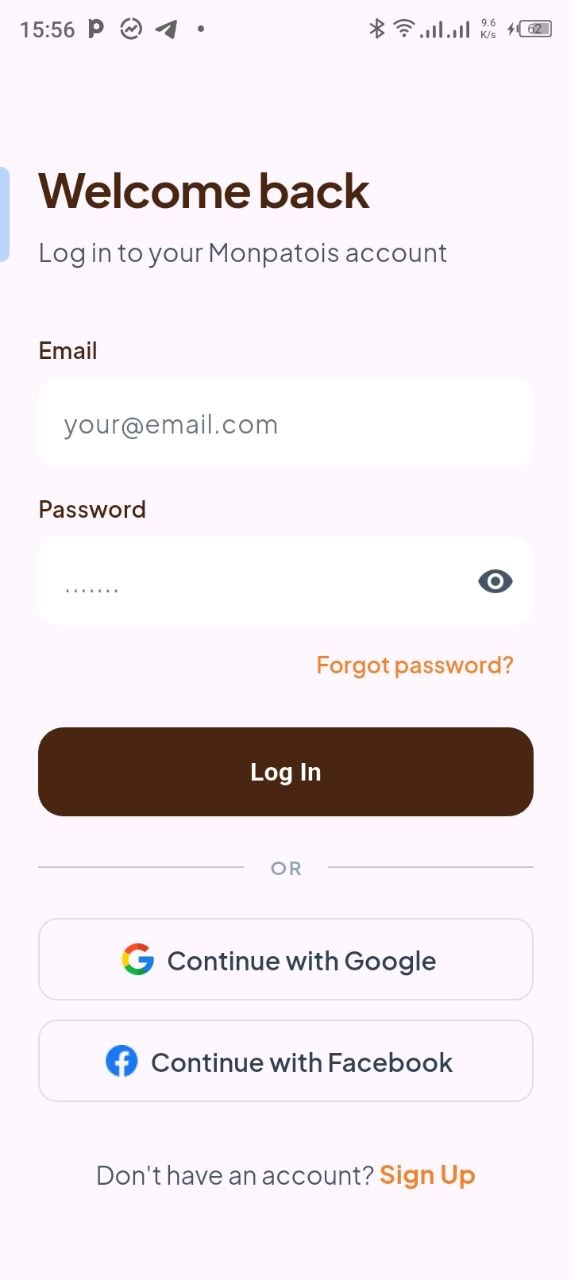
\includegraphics[height=0.82\textheight]{maquette.jpg}
\end{frame}

\begin{frame}{Étape 1 --- Détection des boîtes sur la maquette}
\begin{columns}[T]
\begin{column}{0.32\textwidth}
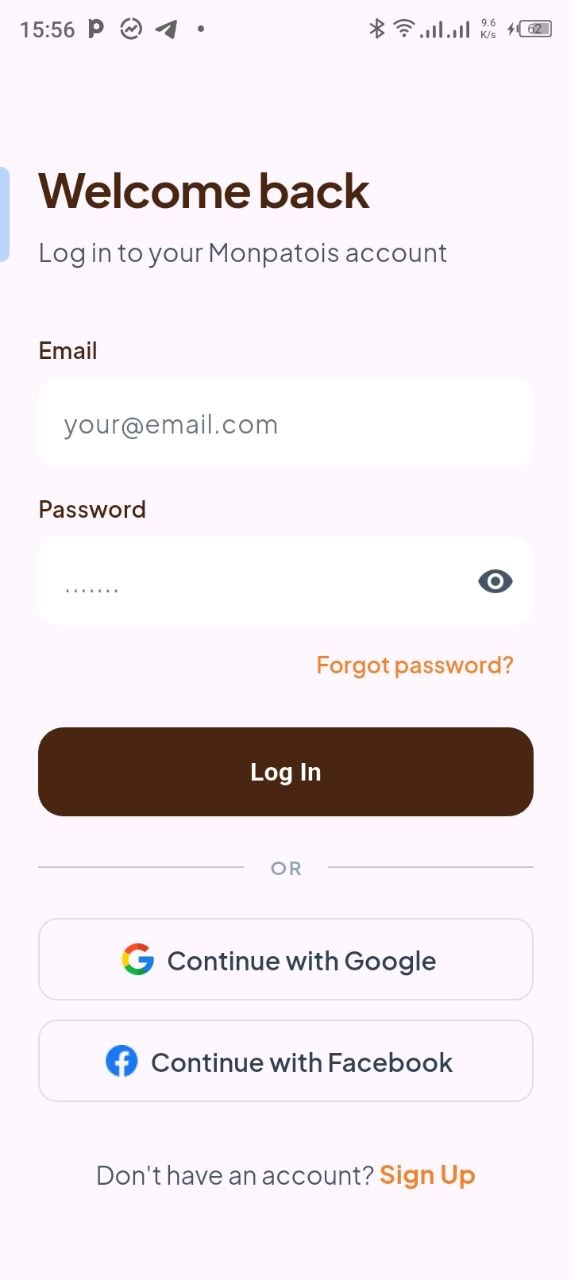
\includegraphics[width=\textwidth]{maquette.jpg}
\end{column}
\begin{column}{0.68\textwidth}
\tiny
\begin{tabular}{@{}clcc@{}}
\toprule
\textbf{ID} & \textbf{Élément} & \textbf{Type} & \textbf{Groupe} \\
\midrule
$b_1$ & Welcome back & Titre & $g_1$ \\
$b_2$ & Log in to your... & Sous-titre & $g_1$ \\
$b_3$ & Email & Label & $g_2$ \\
$b_4$ & your@email.com & Champ & $g_2$ \\
$b_5$ & Password & Label & $g_3$ \\
$b_6$ & •••••• & Champ & $g_3$ \\
$b_7$ & Forgot password? & Lien & $g_4$ \\
$b_8$ & Log In & Bouton & $g_4$ \\
$b_9$ & OR & Séparateur & $g_5$ \\
$b_{10}$ & Continue with Google & Bouton & $g_5$ \\
$b_{11}$ & Continue with Facebook & Bouton & $g_5$ \\
$b_{12}$ & Sign Up & Lien & $g_6$ \\
\bottomrule
\end{tabular}

\vspace{0.3cm}
\normalsize
Chaque élément détecté devient un \textbf{n\oe{}ud} du futur graphe, avec sa position $(x,y)$ mesurée sur l'image.
\end{column}
\end{columns}
\end{frame}

\begin{frame}{Étape 2 --- Calcul de similarité (exemple concret)}
On compare $b_3$ (Email) et $b_4$ (champ) : très proches verticalement.

\[
\text{sim}_{\text{geo}}(b_3,b_4) = e^{-0.04/0.1} \approx 0.67
\qquad
\text{sim}_{\text{sem}}(b_3,b_4) \approx 0.3
\]
\[
\sigma(b_3,b_4) = 0.6 \times 0.67 + 0.4 \times 0.3 = 0.522 \;\; (> \theta = 0.5) \;\Rightarrow\; \textbf{arête tracée}
\]

\vspace{0.3cm}
On compare maintenant $b_3$ (Email) et $b_9$ (OR) : très éloignés sur l'écran.

\[
\text{sim}_{\text{geo}}(b_3,b_9) = e^{-0.40/0.1} \approx 0.018
\qquad
\sigma(b_3,b_9) \approx 0.051 \;\; (< \theta) \;\Rightarrow\; \textbf{pas d'arête}
\]

\begin{block}{Principe}
On répète ce calcul pour \textbf{toutes les paires} de boîtes détectées. Seules les paires dont $\sigma \geq \theta$ sont reliées dans le graphe.
\end{block}
\end{frame}

\begin{frame}{Étape 3 --- Le graphe  obtenu}
 
\centering
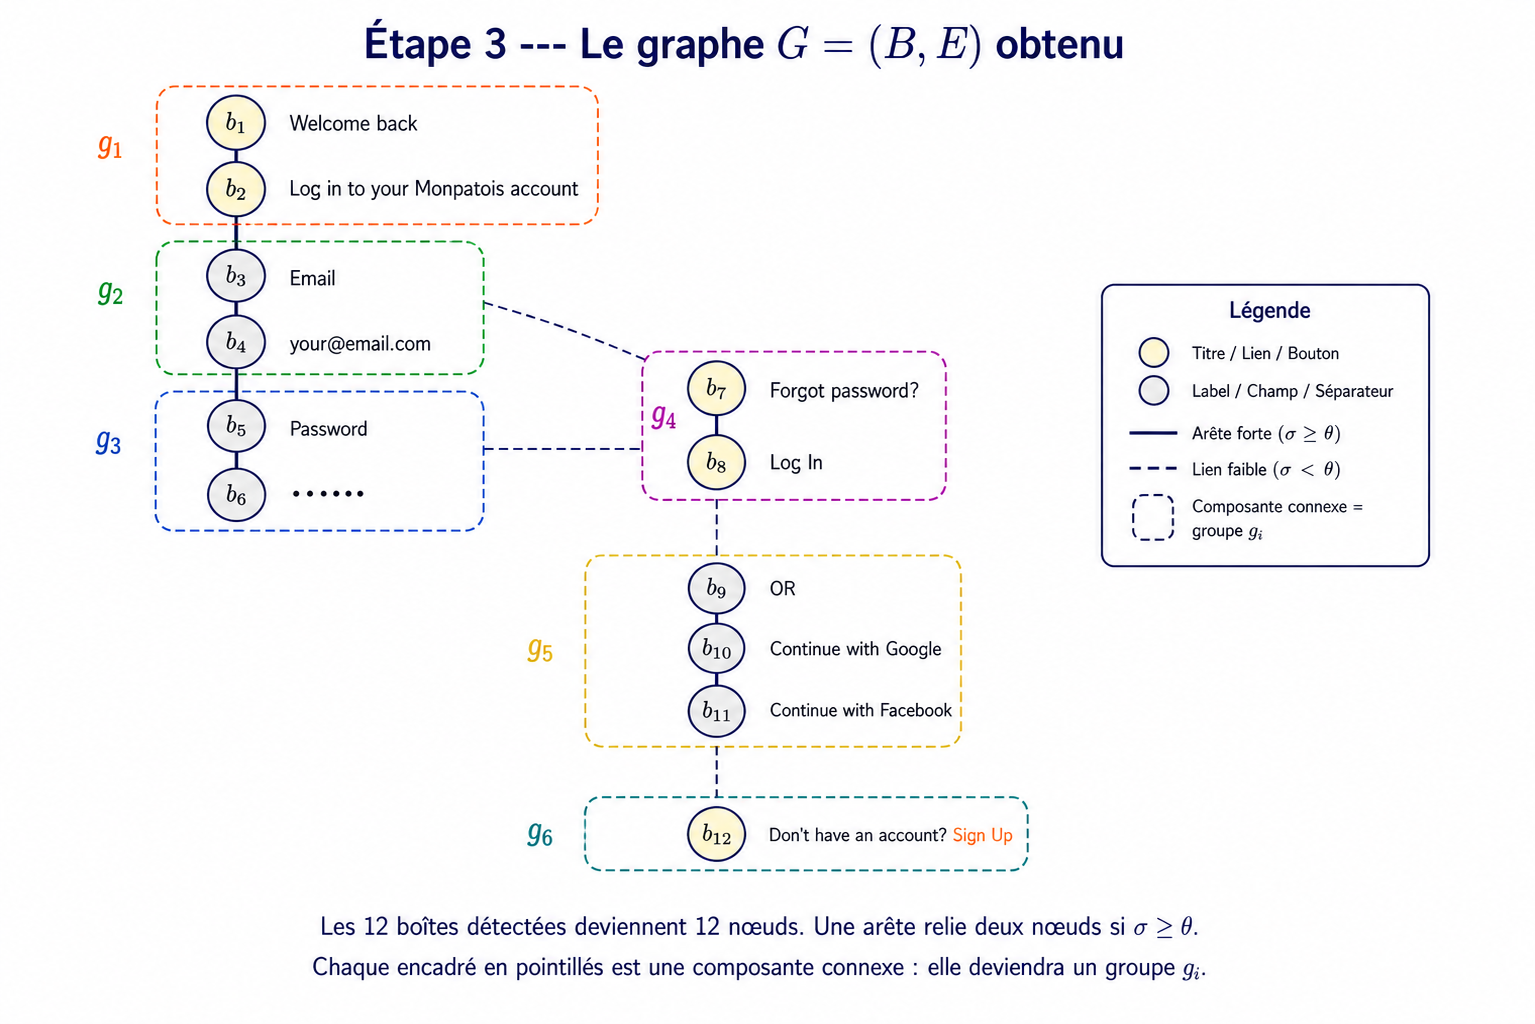
\includegraphics[height=0.82\textheight]{resultat.png}
\end{frame}

\begin{frame}{Étape 4 --- Des groupes vers le modèle}
\begin{block}{Ce qu'on obtient}
Le graphe s'est transformé en \textbf{6 groupes logiques} :
\end{block}
\small
\begin{itemize}
    \item $g_1$ = \{Welcome back, sous-titre\} --- en-tête
    \item $g_2$ = \{Email, champ email\} --- champ formulaire
    \item $g_3$ = \{Password, champ password\} --- champ formulaire
    \item $g_4$ = \{Forgot password?, Log In\} --- actions
    \item $g_5$ = \{OR, Google, Facebook\} --- connexion sociale
    \item $g_6$ = \{Sign Up\} --- pied de page
\end{itemize}

\vspace{0.3cm}
\end{frame}

\begin{frame}
\centering
{\Large\color{navy}\textbf{Merci}}
\end{frame}

\end{document}